\chapter{Experimental Overview of the LHC and CMS}

\label{chapter:expOverview}
The Large Hadron Collider (LHC) is the latest (and most powerful) collider built
to date. It sits beneath the French-Swiss border outside of Geneva, in the
tunnels that were originally used to house LEP. It was designed for
proton-proton collisions, with designed center-of-mass energies of up to 14 TeV.
These design center of mass energies will not be reached until after a series of
hardware updates which are currently underway. This thesis uses instead the
collision data collected at 7 and 8 TeV center-of-mass energies.

The LHC houses 4 major detectors, in addition to a handful of secondary
experiments. The Compact Muon Solenoid (CMS) and A Toroidal LHC Apparatus
(ATLAS) are general-purpose detectors that sit roughly across from each other on
the main proton ring. LHCb is a detector specializing in b-physics (the physics
of mesons containing bottom quarks). The fourth major experiment is the A Lead
Ion Collider Experiment, or ALICE. This detector is designed for primary
operation during the LHC's heavy ion collision mode. Additional experiments,
such as TOTEM and LHCf, are smaller in scale, but aim for important measurements
(these in particular aim, respectively, for total pp cross section measurements
and forward neutral pion measurements).

The operation of the LHC is outlined in Section~\ref{section:theLHC}, while CMS
and its subcomponents are explained in detail in Section~\ref{section:cms}.

\section{Definitions of Terminology}

The geometry of the CMS detector is defined such that the $\hat x-$axis points
toward the center of the ring, and the $\hat y-$axis points upward. The $\hat
z-$axis, then, points in the direction of the proton beam circulating
counterclockwise around the ring (when viewed from above). The angle $\phi$ is
measured up from the $\hat x-$axis in the xy plane, while the polar angle
$\theta$ is measured up from the $\hat z-$axis. The polar angle is often used to
describe the particle's \emph{pseudo-rapidity}, $\eta$, defined as:
\begin{equation*}
    \eta = - \ln \left(\tan ( \frac{\theta}{2}) \right) 
\end{equation*}.

The rate of particles per unit area available for collisions is called the \emph{instantaneous
luminosity}, \instlum:
\begin{equation}
    \instlum = \frac{f_{rev} n_b N_b^2 \gamma_r}{4\pi \epsilon_n \beta*} F
\end{equation}
where $f_{rev}$ is the frequency of the particles' revolution, $n_b$ is the number of
bunches present in the beam chain, $N_b$ is the number of particles in each
bunch, $F$ is a geometric factor resulting from the crossing angle of the beams,
$\gamma_r$ is the relativistic gamma factor, and $\epsilon_n$ is the normalized
beam emittance in the transverse direction. These beam parameters are set by the
machine's operating abilities, with the denominator interpretable as how tightly
squeezed the beam is in the x-y plane (as it travels along a z-axis).
%\temp(what are these values at the LHC?)

%\temp(Transverse momenta?)
%\temp(Invariant mass?)
%\temp(Or just stuff relevant to detector descriptions?)

\section{The Large Hadron Collider}
\label{section:theLHC}
The proton beams which feed the collisions in the LHC start in a modest hydrogen
tank at the beginning of the Linac2 linear accelerator. The hydrogen atoms are
stripped of their electrons, becoming protons that are accelerated along the
linear accelerator up to an energy of 50 MeV. The protons are then injected into
the Proton Synchrotron Booster (PSB), where they are further boosted to 1.4 GeV.
The next step are the Proton Synchrotron (PS) and Super Proton Synchrotron
(SPS), which accelerate them to 25 and 450 GeV respectively. 

After the SPS, the proton beams are injected into the LHC ring, with beams
circulating in opposite directions through the 27 kilometer circumference ring.
Here they are accelerated to their final energy, stored, and steered toward
collision.  The accelerator chain is depicted in Figure~\ref{fig:lhcChain}. The
acceleration of the protons at each stage is done using RF (radio frequency)
cavities. Inside of these cavities, the carefully time oscillations of
electromagnetic fields `push' the proton bunches to accelerate them. The timing
of these oscillations also help keep the bunches together, as protons lagging
slightly behind the majority receive a larger relative boost than protons in the
bulk.  There are sixteen of these cavities in the LHC ring, with eight being
used for each of the beams. The operating frequency of 40 MHz is driven by the
nominal LHC bunch spacing, allowing for bunch spacings of 25~ns.

\begin{figure}[h]
\centering
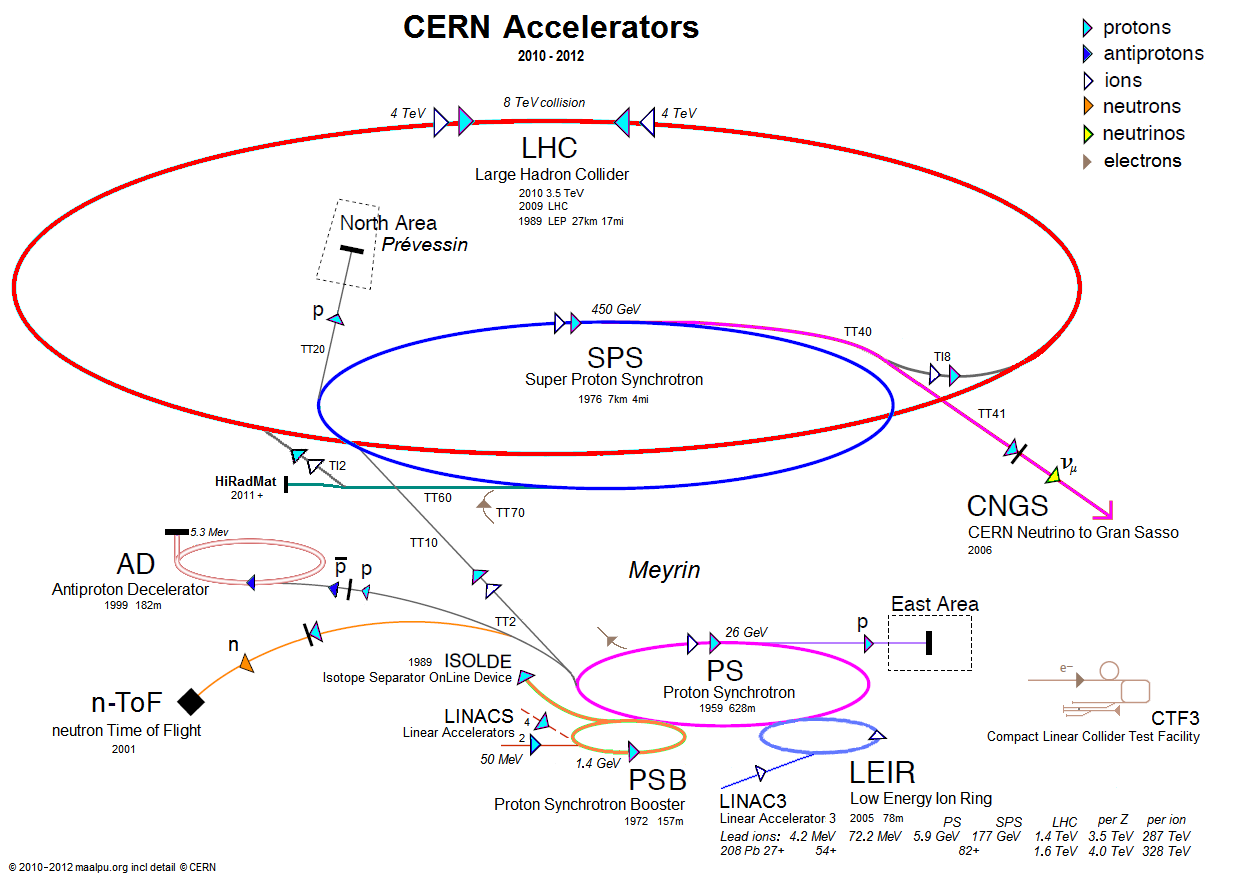
\includegraphics[width=0.90\textwidth]{LHC_chain}
\caption[The LHC accelerator chain.]{The LHC acceleration chain. Protons start in the Linac2 accelerator
(bottom, center), are accelerated through the PSB, PS, and SPS before being
injected into the LHC ring.}
\label{fig:lhcChain}
\end{figure}

The beams are steered using a series of 1232 superconducting dipole magnets, with magnetic
fields of up to 8.3 Tesla. Because there are two proton beams within the LHC ring
circulating in opposite directions, the dipoles have a twin-bore design. In this
setup, there are two beam pipes, with each pipe having its own set of coils to
produce the steering field. In addition to the dipoles, there are 400 quadrupole
magnets which focus the proton bunches. 
%It is only near the interaction regions inside of the detectors that the two beams share one beam
%temp more about magnets?

\begin{table}[h]
\centering
\begin{tabular}{|c|c|c|c|}
\hline
    & 2011 & 2012 & Design \\
\hline
Center of mass collision energy (TeV) & 7 & 8 & 14 \\
Peak Inst. Lumi. ($cm^{-2}~s^{-1}$) & 3.54 & 7.67 & 1.0 \\
Peak Colliding Bunches & 1331 & 1380 & 2808 \\
%Protons per bunch & & & $1.15 \cdot 10^{11}$ \\
Maximum pileup & 16.15 & 34.55 & 19.02 \\
Maximum recorded data, single fill & 118.0 \pbinv & 238.9 \pbinv & -\\
\hline
\end{tabular}
\caption[Machine specifications for the LHC.]{Peak Machine Specifications for 2011 and 2012 proton-proton collisions
at the LHC.} 
%source: https://twiki.cern.ch/twiki/bin/view/CMSPublic/LumiPublicResults#Proton_proton_reference_run_for
%source: https://edms.cern.ch/file/445830/5/Vol_1_Chapter_2.pdf
\label{tab:lhcPerformance}
\end{table}

\begin{figure}[h]
\centering
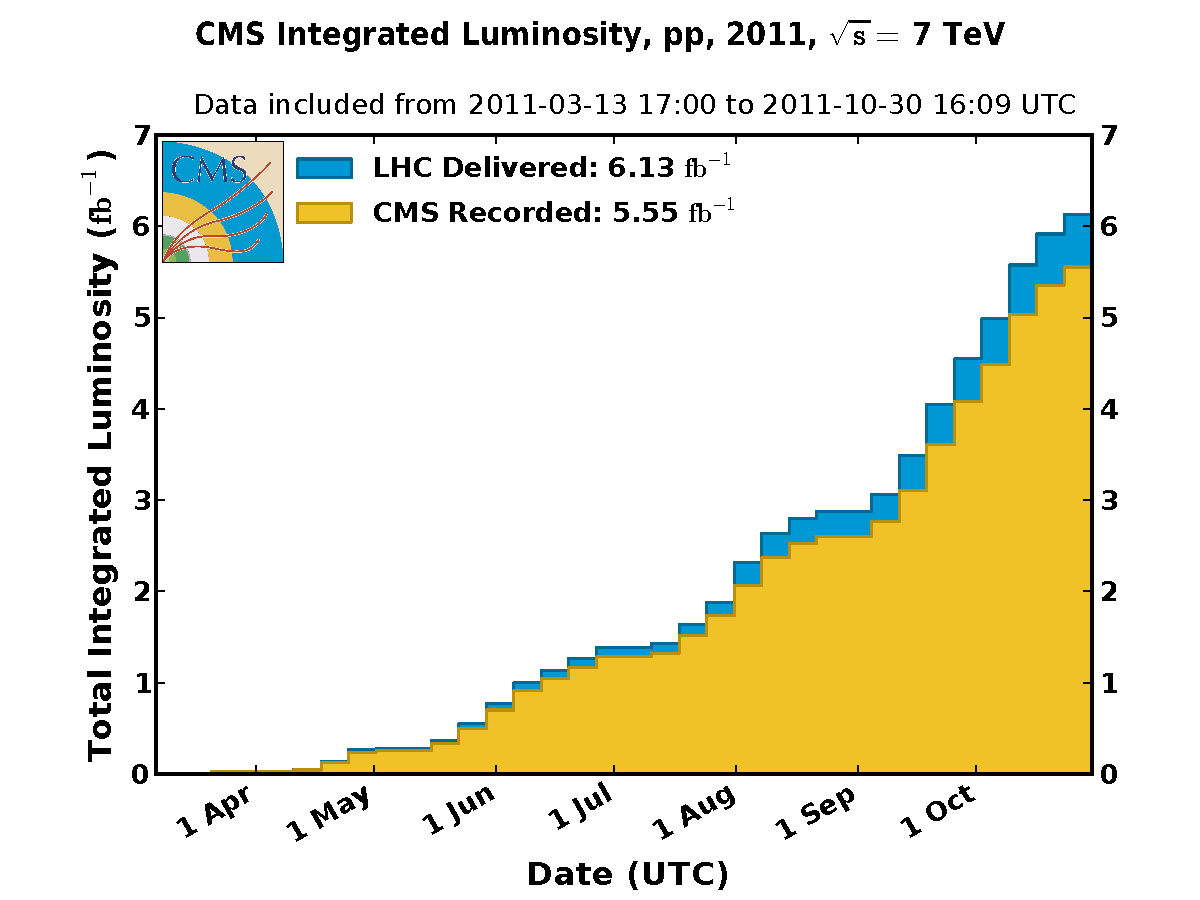
\includegraphics[width=0.45\textwidth]{ppLumi_per_week_2011}
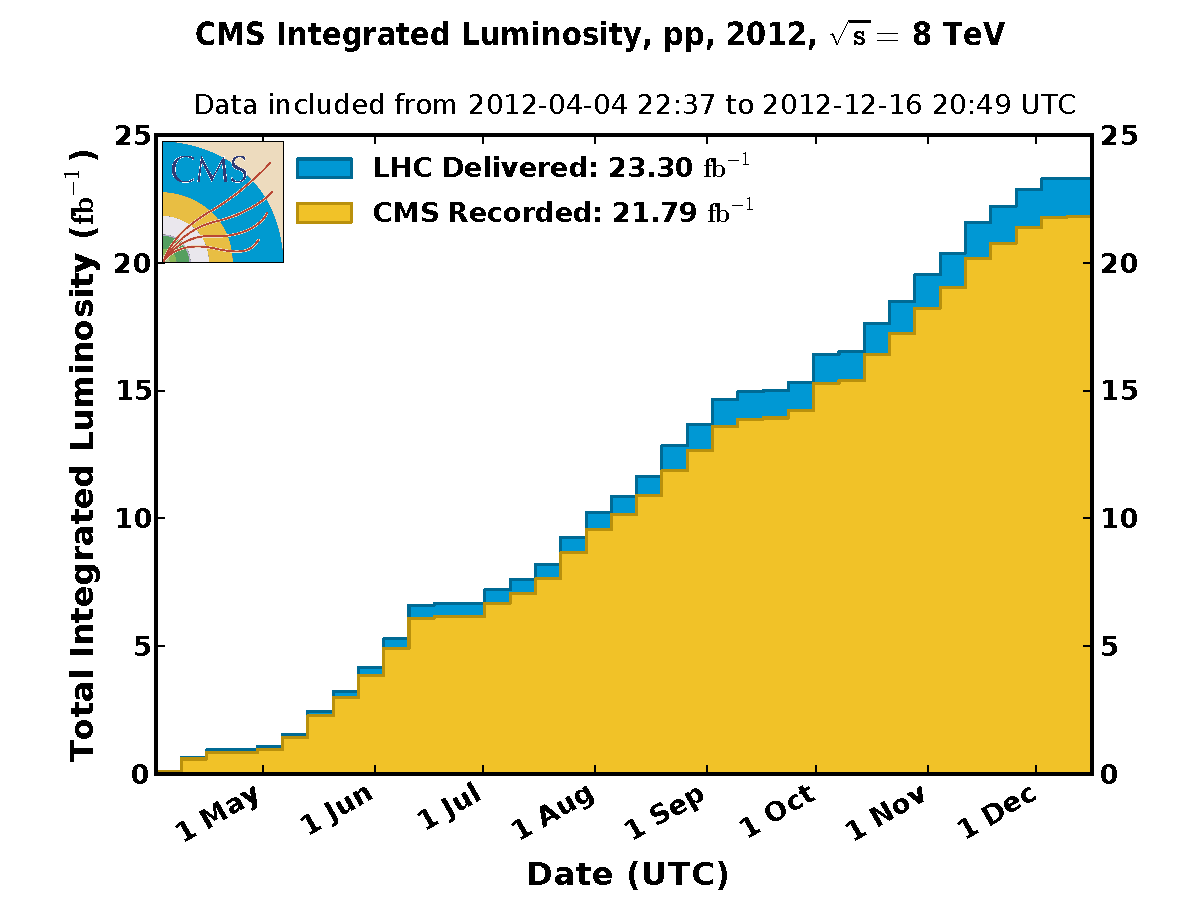
\includegraphics[width=0.45\textwidth]{ppLumi_per_week_2012}
\caption[The amount of intergraled luminosity at the LHC in 2011 and 2012.]{The amount of integrated luminosity delivered by the LHC and recorded
by the CMS detector in each week of 2011 (left) and 2012 (right).}
\label{fig:dataCollected}
\end{figure}

\section{The Compact Muon Solenoid detector}
\label{section:cms}
The Compact Muon Solenoid, or CMS, is one of the two multi-purpose detectors on
the LHC experiment. It is immense, both in size and scope. It is 21.6 meters
long, 14.6~m in diameter, and weighs in at about 12,500~t. The various
components where primarily built on the surface before being lowered into the
detector cavern, 100~m below ground. CMS sits at the LHC ``Point 5,'' located
near the French town of Cessy, roughly on the opposite side of the ring from
ATLAS and the main CERN campus. 

Like many detectors, CMS features an inner tracking system (for determining the
momenta of charged particles), a magnetic solenoid (in order to bend the
trajectory of charged leptons for accurate momenta measurements),
electromagnetic and hadronic calorimeters (for measurements of particle energy),
an outer muon system (for detection of muons, which tend to pass through the
inner components without significant interaction). CMS is unique in the
placement of the magnet outside of the calorimetric elements: the
`compact'-edness of the tracker and calorimeter allow these components to fit
inside the magnet. In traditional detectors, the magnet is placed immediately
outside of the tracking system, meaning that particles can interact (and lose
energy) in the material of the magnet before reaching the calorimeters.

An isometric diagram of the detector is shown in figure~\ref{fig:cmsExploded},
while a cutaway showing a fraction of the xy-plane of the detector with a
simulated collision interaction is shown in figure~\ref{fig:cmsCutaway}

\begin{figure}[h]
\centering
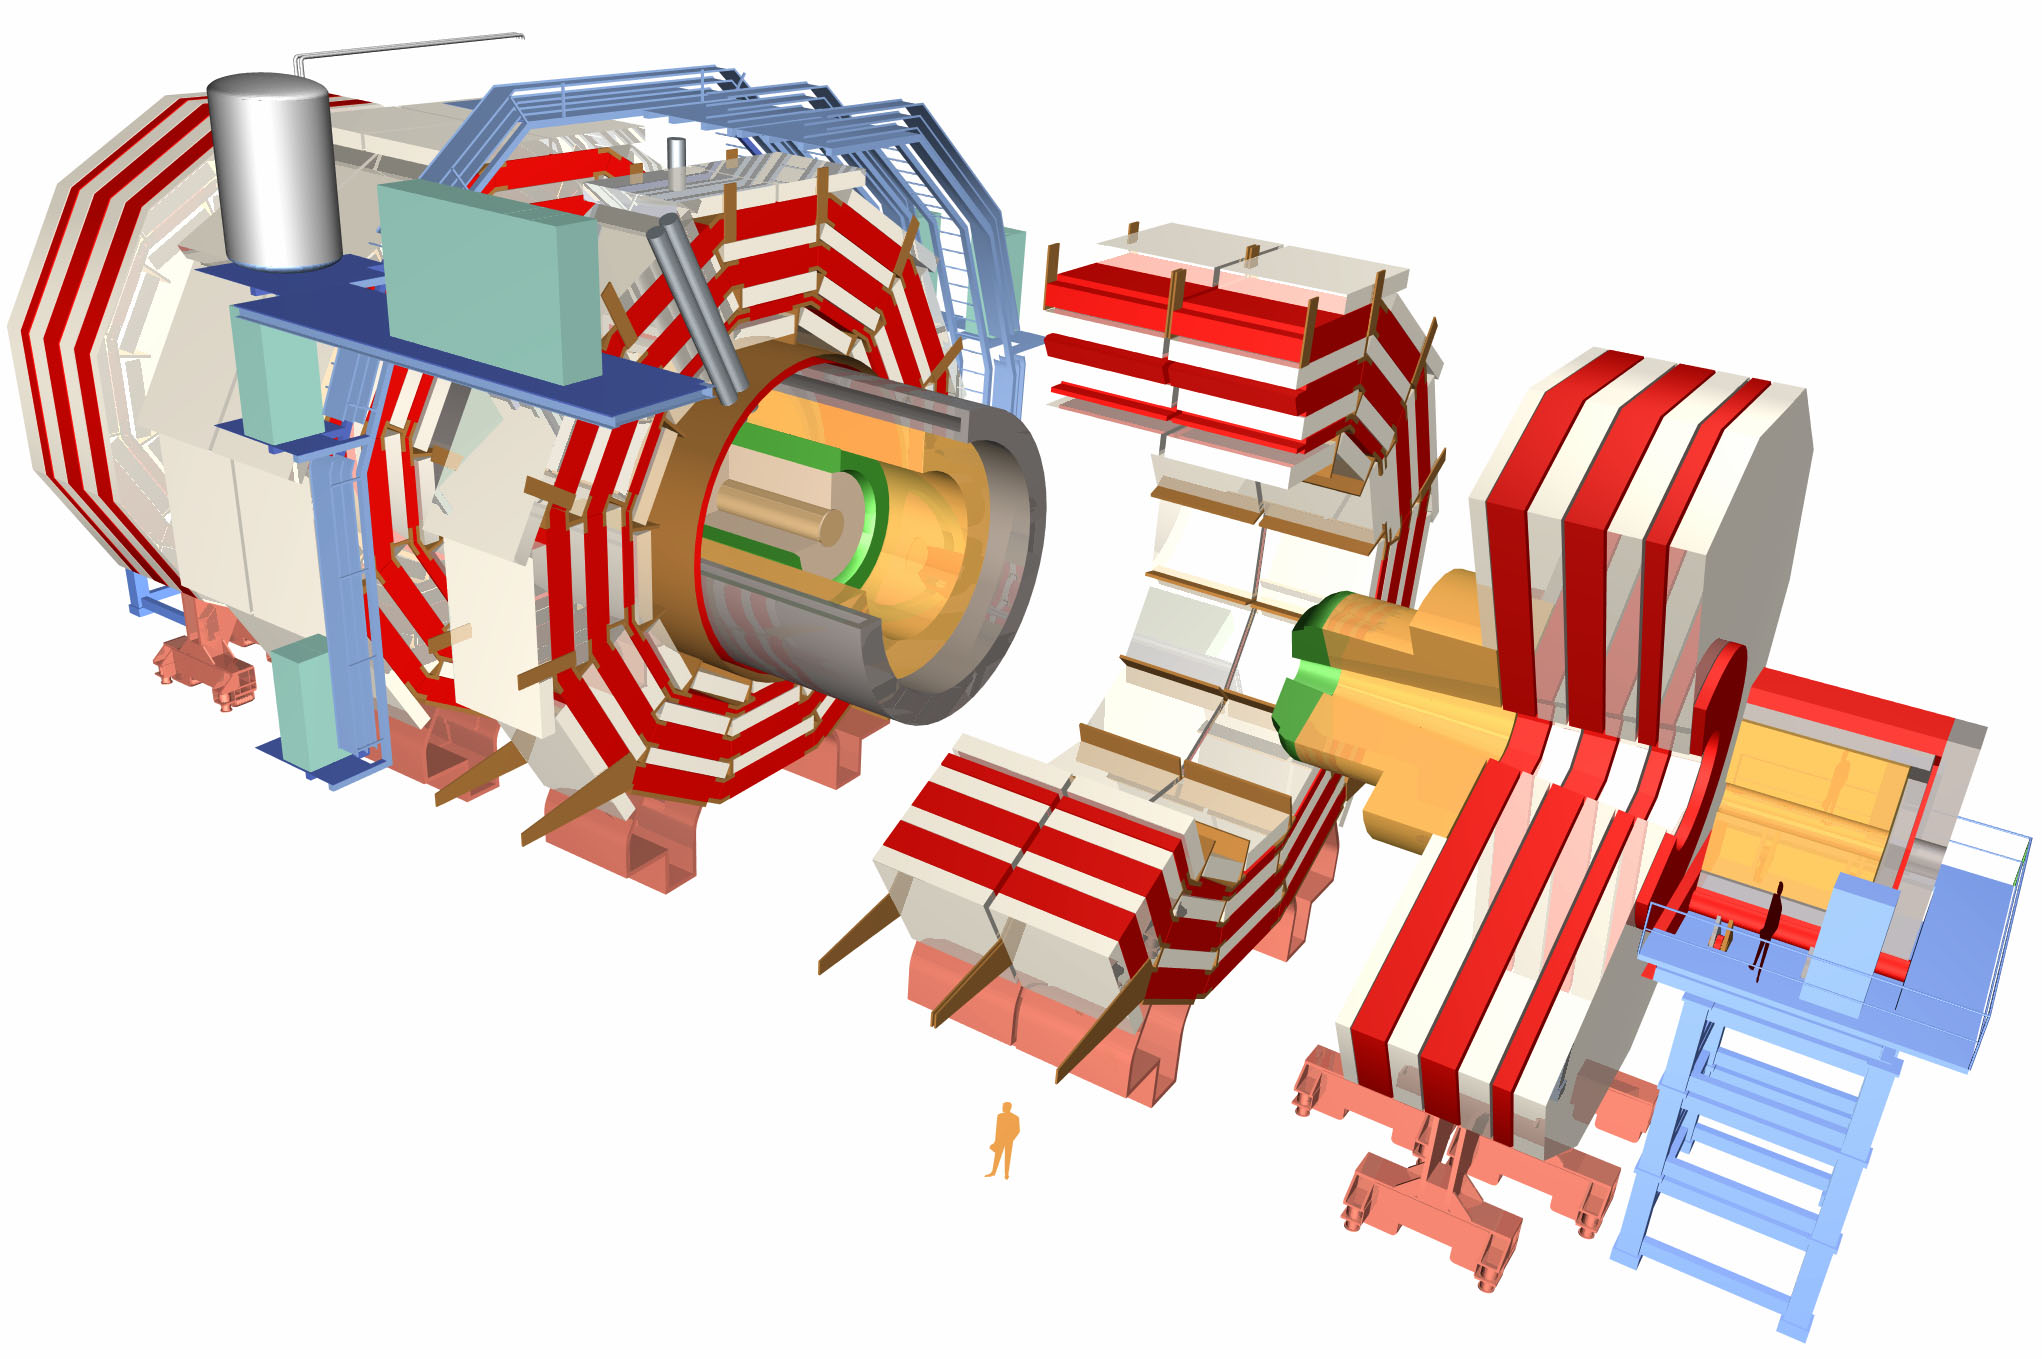
\includegraphics[width=0.6\textwidth]{cms_exploded}
\caption[Isometric view of CMS]{An exploded isometric view of the CMS detector, showing the overall
geometry and layering of the components.}
\label{fig:cmsExploded}
\end{figure}

\begin{figure}[h]
\centering
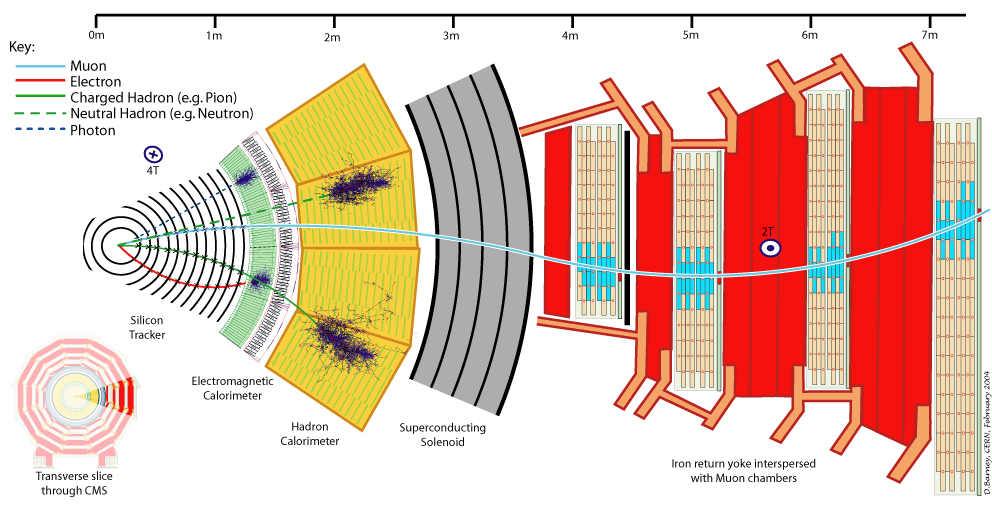
\includegraphics[width=0.8\textwidth]{cms_cutaway}
\caption[A cutaway slice of the CMS detector.]{A diagrammed slice of the CMS detector, showing the components' nesting
and the interactions of different particle types with the subcomponents.}
\label{fig:cmsCutaway}
\end{figure}

\subsection{Tracker}
The innermost component of the CMS detector is the silicon tracking system. Its
role in particle detection is twofold: to provide accurate spatial measurements
for primary and secondary vertices and to accurately measure the curved
trajectories from the charged particles. The tracker system sits just outside
the beampipe, with detecting area starting at a radius of 4.4~cm, extending to
radial distance of 1.1~meters. The system is 5.8~m in length, with disks at
either end of the cylinder to provide coverage in the pseudorapidity range
$|\eta|<2.5$.  The system is made of two subcomponents: the \emph{pixel
detector} and the \emph{silicon strip detector}. In both systems, the primary
technology used for particle detection is reverse-biased np silicon junction. As
charged particles pass through the silicon, ionization deposits in the substrate
cause a depletion current which is read out electronically. The use of this
silicon technology allows very thin sensors to be used, minimizing particles'
interaction with non-detection material while providing the extremely quick
detection response times required by the high collision rates provided by the
LHC. The layout of the tracker is provided in Figure~\ref{fig:trackerLayout}.

\begin{figure}[h]
\centering
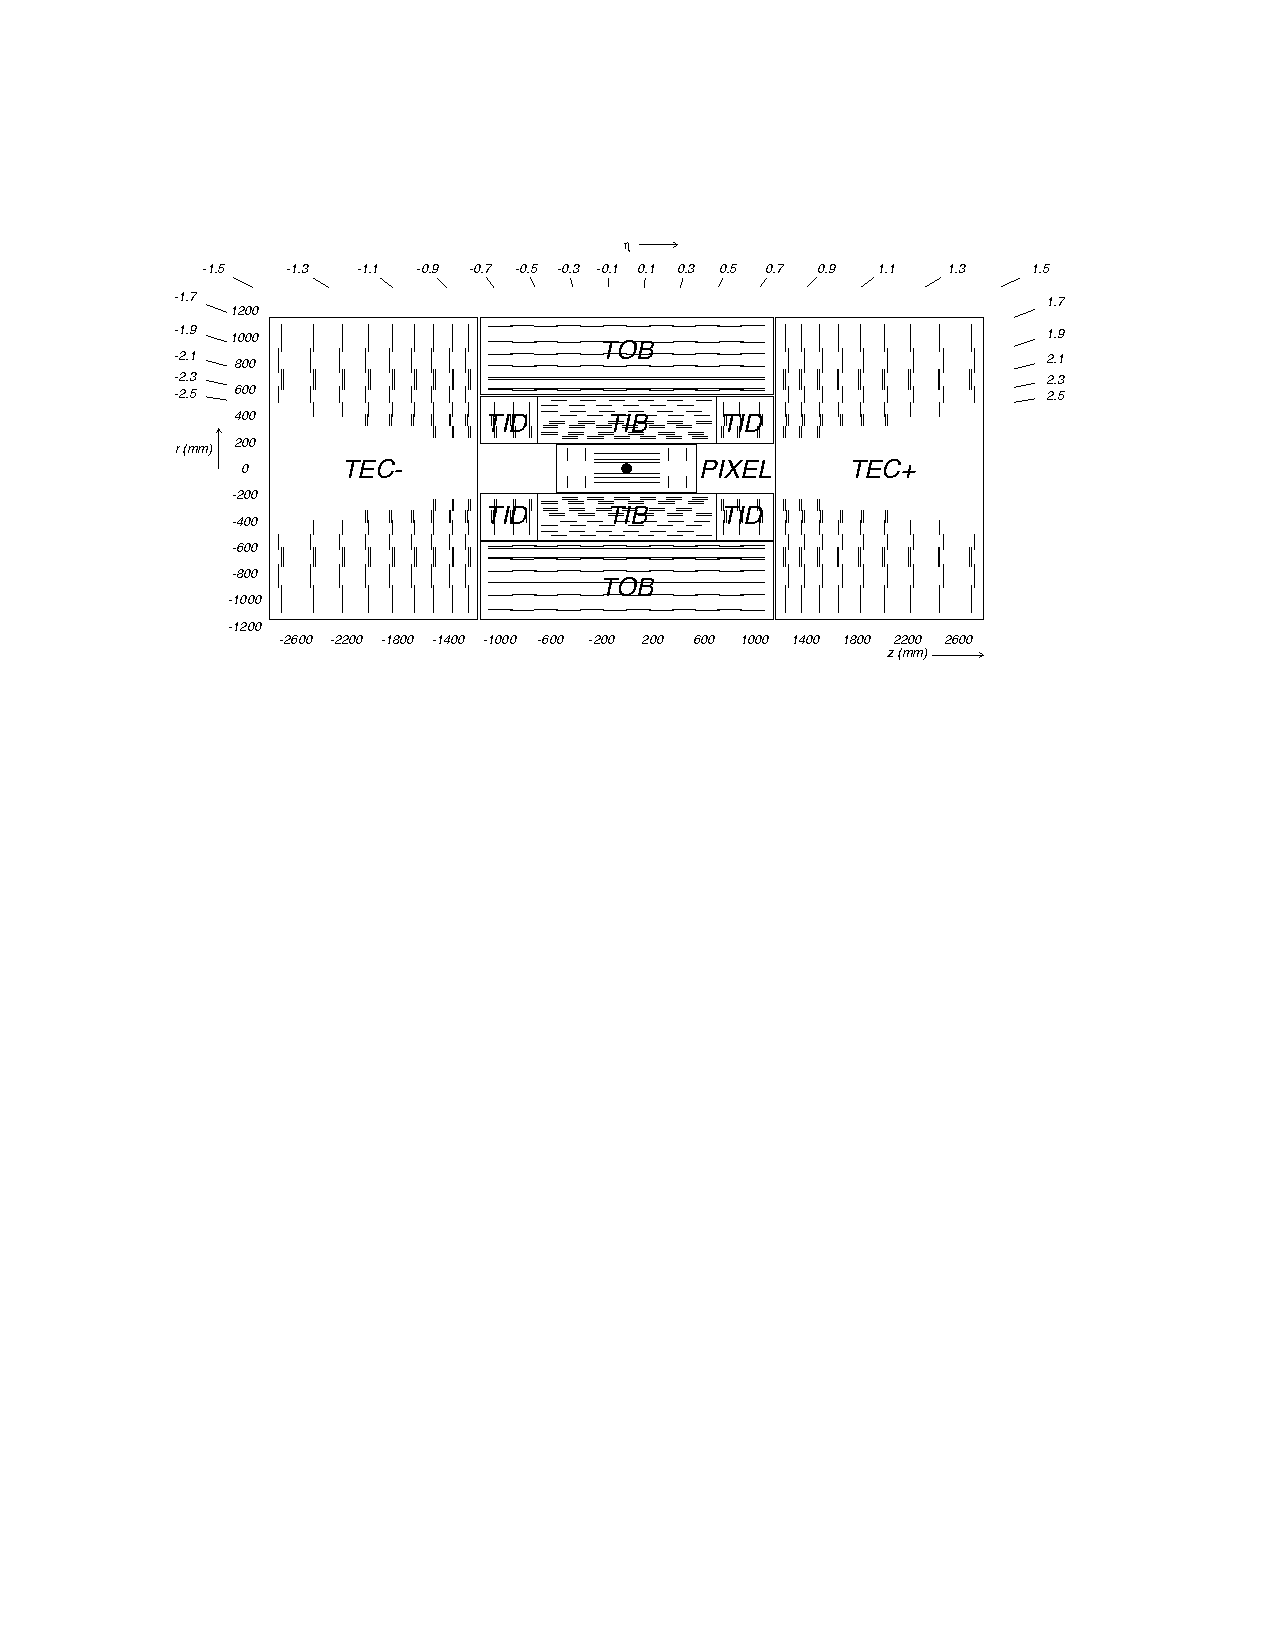
\includegraphics[width=0.8\textwidth]{tracker_layout}
\caption[The geometry of the CMS tracking system.]{The geometry of the inner tracking system of CMS. There are three
central layers of pixel detectors, with an additional two in the forward disk.
There are ten central layers of strip detector, with an additional 3+9 in the
disks.}
\label{fig:trackerLayout}
\end{figure}

The three innermost layers compose the so-called pixel detector,
consisting of 100 $\times$ 150 $\mu m^2$ silicon pixels. These pixels provide
excellent spatial granularity in the most densely occupied region. The primary
purpose of these pixel layers are to provide very fine position measurements in
all three dimensions. The pixels provide measurements in the $r-\phi$ plane with
a resolution on the order of $10 \mu m$ and in the $r-z$ plane to about $20 \mu
m$.  This fine granularity provides the ability to pinpoint, in three
dimensions, the location of primary and secondary vertices. Secondary vertices
are the result of decays of short-lived particles that are born in the primary
interaction (such as a b-quark traveling a short distance before hadronizing
into a jet).  In total, there are 66 million pixels, providing about 1$m^2$ of
detecting area. The position resolution provides CMS with the ability to
accurately locate primary collision vertices, critical both in momenta
measurements of curved tracks and pile-up rejection. Both of these benefits are
discussed in further detail in later chapters of this thesis.

The next 10 layers of the tracking system are covered by the silicon strip
detector, extending to an outer radius of 1.1 m. Because of the lower track
occupancy in this region, the detecting components are not designed to have as
fine a granularity along the $\hat z-$direction.
The strips located in the barrel region  measure $10 cm \times 180 \mu$m in the
inner four layers, known as the tracker inner barrel (TIB), and $25 cm \times
180 \mu $m in the outer six layers (the tracker outer barrel, or \emph{TOB}).
The strip detector subsystem is completed in the more forward endcap regions by
the tracker inner disks (\emph{TID}) and tracker endcaps (\emph{TEC}). 

The information from the pixel and strip detectors are combined to recreate the
path of the charged particles. Because the tracker sits inside of a 3.8~T
magnetic field, the particle paths are curved, allowing measurements of the
momenta through the Lorentz equation:
\begin{equation}
    p = q B R
\end{equation}
where q is the particle's charge, B is the strength of the magnetic field, and R
is the radius of curvature. Particles with higher momenta have as less visible
curvature within the detector and as a result have a larger momenta resolution:
\begin{equation}
    \frac{\sigma(p_T)}{p_T} = p_T \cdot 0.015\% \oplus 0.5\%,  (|\eta|<1.6)
\end{equation}
\begin{equation}
    \frac{\sigma(p_T)}{p_T} = p_T \cdot 0.05\% \oplus 0.5\%,  (1.6 < |\eta| < 2.5)
\end{equation}
The charged particles in this analysis are typically in the 10-50 GeV range,
giving them resolutions on the at the sub-percent level (or a few percent in the
more forward regions).

\subsection{Electromagnetic Calorimeter}
%how does it actually MEASURE energy? IAR 01.May.2013
The next detector component that a particle encounters on its journey outward
through the detector is the electromagnetic calorimeter (\emph{ECAL}). This detector is
designed to capture all of the energy of the electrons and photons produced in
the collisions (or subsequent decays). 

The calorimeter is composed of over 76,000 lead tungstate (PbWO\textsubscript{4})
crystals. As electromagnetic particles pass through these crystals, they produce
electromagnetic showers. The light from these showers is amplified and collected
by avalanche photodiodes in the barrel region and vacuum phototriodes in the
endcap regions. The use of PbWO\textsubscript{4} crystals was motivated by
their radiative resistance, light response, density, and the resulting
compactedness of the calorimeter as a whole.  The dense crystals ($8.28 g/cm^3$)
result in an extremely short radiation length of 0.89$cm$ and a very small
Moliere radius ($2.2 cm$). The geometry of the crystals is designed to utilize
these characteristics, with typical sizes being $22\times22 mm$ at the front
face, $26\times26 mm$ at the rear face, and $230 mm$ in length. As a result,
particles are almost guaranteed to interact somewhere along the crystal length
(traversing roughly 26 radiation lengths), with the resulting EM showers leaking
minimally out of one or two crystals. In addition to the excellent spatial gains of the
crystals, they are additionally very quick. The scintillation decay time is
sufficiently short so that roughly 80\% of the light is emitted within the 25 ns
corresponding to the nominal LHC bunch cross rate. 

The crystals are bundled into submodules, which are grouped into modules which
vary in makeup in order to optimize the uniformity of the crystal coverage.
These modules are then grouped into supermodules, which consist of 1700
crystals, with a 20 crystal coverage in $\phi$ and an 85 crystal coverage in
$\eta$.

The ECAL is composed of of three primary subcomponents: the barrel (\emph{EB}),
the endcap (\emph{EE}), and the preshower (\emph{ES}). The EB covers the area
within $|\eta|<1.479$ and contains the bulk (61,200) of the PbWO\textsubscript{4}
crystals. The EE covers the forward regions, with a pseudorapidity coverage of
$1.56 < |\eta| < 3.0$ and contains 7234 PBWO\textsubscript{4} in each endcap.
The crystals in the endcaps are slightly larger than those in the EB, with a
front face of $28.62\times28.62 mm$ and a rear face of $30 \times 30 mm$ with a
length of 220 mm. The ES sits just in front of the endcap crystals, providing an
$|eta|$ coverage from 1.653 to 2.6. It is composed of
a layer of lead radiators to produce electromagnetic showers, with silicon strip
detectors behind to measure the deposits. The purpose of the ES is primarily to
detect forward neutral pions, in order to distinguish the neutral mesons from
photons. The layout of the ECAL is pictured in Fig.~\ref{fig:ECAL_geometry}.

\begin{figure}[h]
\centering
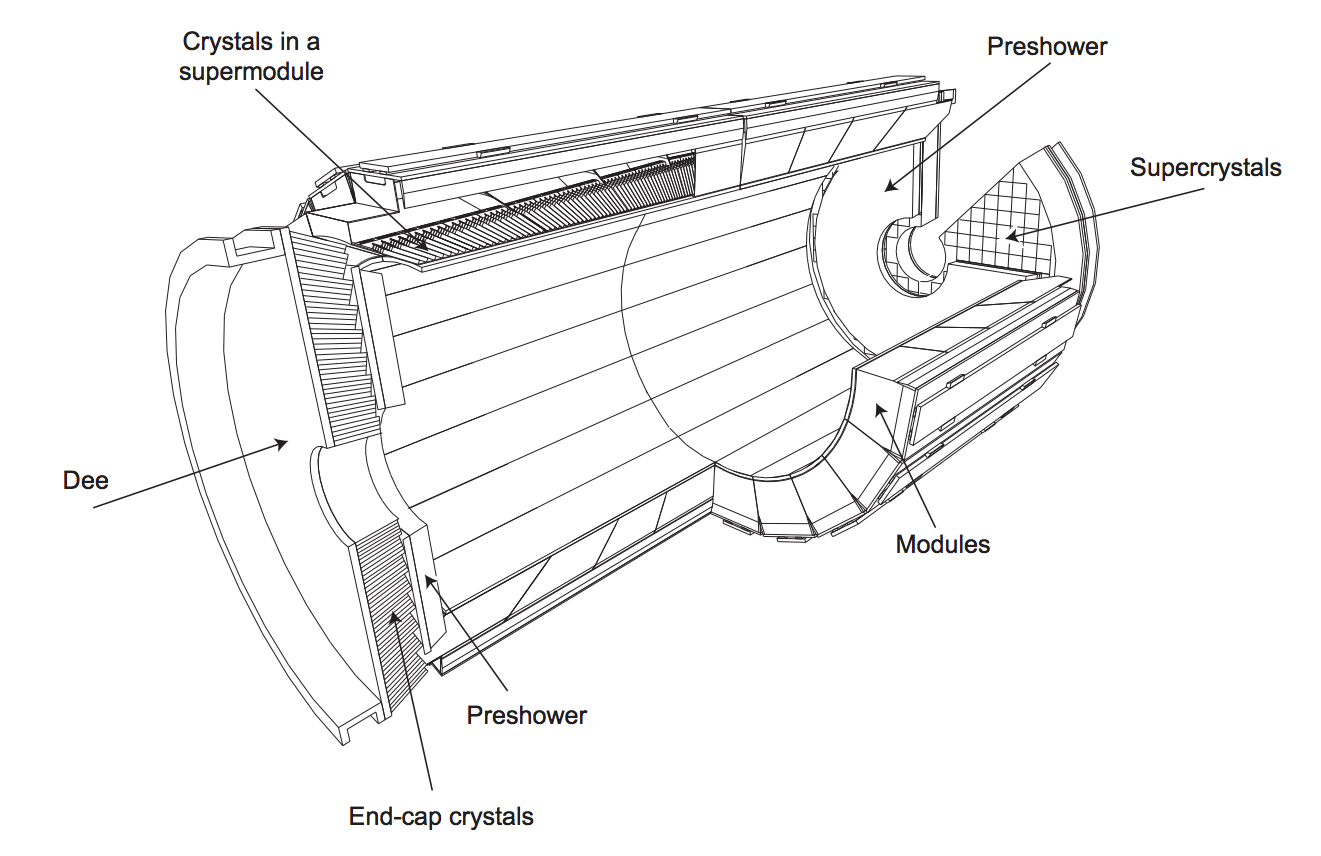
\includegraphics[width=0.8\textwidth]{ECAL_geometry}
\caption[The geometry of the CMS electromagnetic calorimeter.]{The geometry of the CMS Electromagnetic Calorimeter, diagramming the
crystals, modular structure, and overall layout of the EB, EE, and ES
subcomponents.}
\label{fig:ECAL_geometry}
\end{figure}

Because of the high granularity, the ECAL provides excellent spatial resolution
for a calorimeter. However, the crystals' beam-facing orientation combined with
the lack of a segmented depth setup means that there is no information provided
about the angle of the particles as they enter the calorimeter. Thus, the
positional information is limited to the size of the crystals themselves.

The radiation due to the large flux of particles through the detector has the
effect of harming the overall transparency of the crystals. As a result, the
energy measurements tend to drift over time, resulting in systematic deviations
of energy measurements (and larger variations in response from crystal to
crystal).. This is handled using a laser calibration system, which provides a
set of corrections and calibrations which evolve over the length of a run.

The energy measurement of the ECAL is energy-dependent:
\begin{equation}
    \left(\frac{\sigma(E)}{E}\right)^2 =
        \left(\frac{2.8\%}{\sqrt{E}}\right)^2+\left(\frac{0.12}{E}\right)^2+\left(0.30\%\right)^2
\end{equation}
with the energy is provided in~GeV.  The first term is due to the inherent
statistical nature of the EM showering processes, while the second is due to
electronic noise. The third term is due to non-uniformity in the geometric
layout of the detector and calibration uncertainties.

\subsection{Hadronic Calorimeter} 
%still needs more information about the measurements?  IAR 01.May.2013
The Hadronic Calorimeter (or \emph{HCAL}), which sits outside of the ECAL, is
built with the intent to measure the energy of the hadronic jets. It is
important in the measurements of missing transverse energy, which is energy
carried away by non-interacting particles (such as neutrinos or some kinds of
exotic particles). In addition to providing key measurements of hadronic energy,
the HCAL also provides a useful layer of discrimination for potentially fake
electromagnetic particles. If an ECAL deposit is associated with an HCAL
deposit, there is a good chance that the particle was a hadron which interacted
with a nucleus in the ECAL (since truly electromagnetic particles like the
electron will deposit 100\% of their energy in the ECAL).

In addition to its inherent value to jet studies and missing transverse energy
\emph{ME\textsubscript{T}} calculations, the HCAL is also key in measuring the
amount of pileup present in a collision. As most analyses are sensitive to the
number of soft interactions underlying their events of interest, it is important
to account and correct for the energies and compositions of these pileup events.
The HCAL, with its wide coverage in $|\eta|$ provides measurements critical in
these corrections.

The HCAL is a sampling calorimeter, meaning the shower-inducing and energy
measurement components are physically separate media. Like the ECAL, it is split
into barrel and endcap regions (commonly called the HB and HE subcomponents). In
addition, there is a forward hadronic calorimeter (HF), which sits 11~m forward
of the interaction point. Radially, the HCAL fits snugly between the ECAL and
the solenoid, extending from a radius of 1.77~m to 2.95~m. The HB coverage
extends to $|\eta| < 1.305$, while the HE covers $1.305 < \eta < 3.0$. The HF
covers the most forward regions of the detector, covering $3.0 < \eta < 5.0$.
The geometry of the hadronic calorimeter is diagrammed in
figure~\ref{fig:HCAL_geometry}.

\begin{figure}[h]
\centering
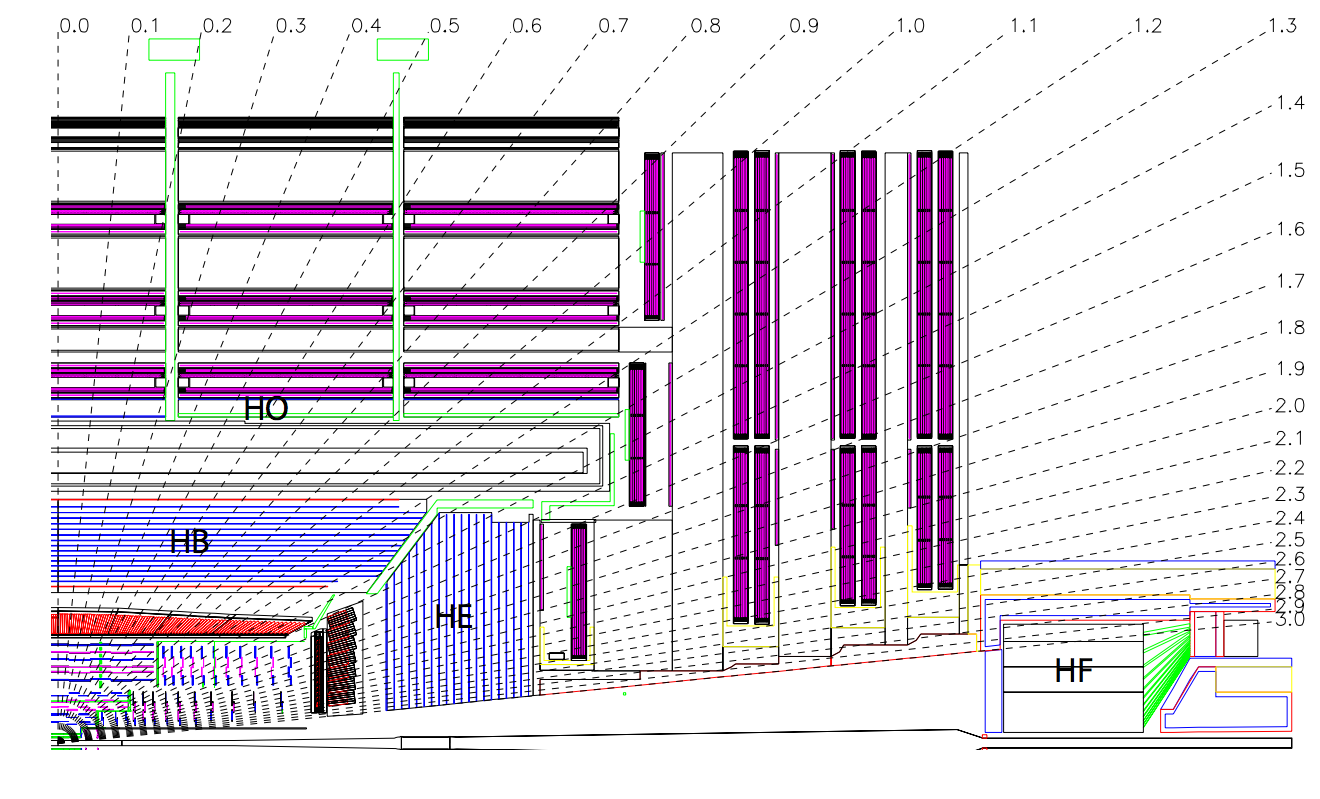
\includegraphics[width=0.8\textwidth]{HCAL_geometry}
\caption[The geometry of the CMS hadronic calorimeter.]{The geometry of a
fraction of the CMS hadronic calorimeter. The HB provides coverage
to $|\eta|<1.3$, the HE covers $1.3<|\eta|<3.0$, and the HF covers
$3.0<|\eta|<5.0$. The dashed lines indicate equal intervals in $\eta$.}
\label{fig:HCAL_geometry}
\end{figure}

The HB and HE subcomponents use interspersed sections of brass (to induce
hadronic showering) and scintillator to measure the resulting energy. In the
more forward HF, where the radiation is a much great concern, the sampling is
done using steel plates coupled with quartz fibers. The interaction length,
$\lambda_i$, of the brass material is 16.42~cm, meaning that a hadronic jet will
be reduced to 1/e of its energy for each 16.42~cm of brass it traverses. The
amount of material increases with the azimuthal angle so that the number of
interaction lengths through the entire HCAL increases from 5.82 $\lambda_i$ to
10.6 $\lambda_i$ at an $|\eta|$ of 1.3. The HE has similar coverage, with about
10 $\lambda_i$ of total material.

The energy resolution for the HCAL is given by:
\begin{equation}
    \left(\frac{\sigma(E)}{E}\right)^2 =
    \left(\frac{90\%}{\sqrt{E}}\right)^2+(4.5\%)^2, HB/HE
\end{equation}
\begin{equation}
    \left(\frac{\sigma(E)}{E}\right)^2 =
    \left(\frac{172\%}{\sqrt{E}}\right)^2+(9.0\%)^2, HF
\end{equation}
where the first term is due to the statistical fluctuations of the hadronic
showering and the second term arises from geometric variations and calibration
uncertainties. 

\subsection{The Magnet}
\label{sub:magnet}
The most striking feature of CMS is the object that gives the detector its name:
the solenoid. The magnet is 6~m in diameter, 12.5~m long, and weighs 220 tonnes.
The superconducting solenoid, consists of 4 layers of NbTi coiling, capable of
producing the 18~kA necessary for the desired 3.8 T magnetic field. This
magnetic field is responsible for causing the trajectory of the charged
particles to bend within the tracker, allowing accurate momenta measurements.
An iron yoke is staggered with layers of the muon chambers, providing the
detector with structural support in addition to feeding a 2~T return field. This
return field allows additional curvature for the muon momenta measurements.

\subsection{Muon chambers}
The outermost component of the CMS detector is the muon system. As suggested by
the name, these subsystems are designed to identify and measure muons. In
addition to the spatial accuracy, it is also critical for the muon systems to be
relatively fast, in order to efficiently trigger on muons within a certain bunch
crossing (as described in~\ref{sub:trigger}). Because muons are so much heavier
than electrons, they largely escape the inner detector components (where the
electrons lose their energy through bremsstrahlung radiation). As mentioned
in~\ref{sub:magnet}, the central portions of the muon system sit in the $\sim$
2~T return field of the solenoid. The field strength, combined with the radial
size of the muon system, allow accurate muon momenta measurements across a wide
spread of energies.

The muon system utilizes three different technologies to achieve its goals of
precise and quick muon measurements. Drift tubes (DTs) are precise, but
relatively slow. This makes them ideal for the barrel region ($|\eta|<1.2$), where particle
rate is expected to be lower. The cathode strip chambers (CSCs) are used
in the more forward regions ($0.9 < |\eta| < 2.4$), where the increased particle
rate requires a quicker technology. Finally, the resistive plate chambers
(RPCs) cover out to $|\eta|<1.6$. RPCs are the quickest technology, but provide
coarser position measurements than either the DTs or CSCs. They are used
primarily for triggering and for resolving ambiguously reconstructed tracks from
other chambers. An overview of the muon system geometry is provided in
Figure~\ref{fig:muonGeometry}.


\begin{figure}[h]
\centering
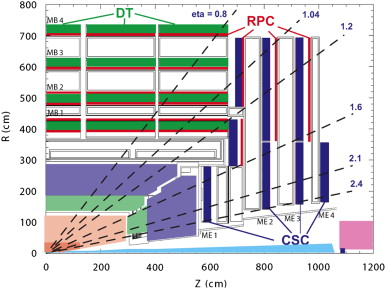
\includegraphics[width=0.6\textwidth]{muon_geometry}
\caption[The geometry of the CMS muon system.]{The geometry of the muon system, composed of the drift tubes (DTs),
cathode strip chambers (CSCs), and resistive plate chambers (RPCs).}
\label{fig:muonGeometry}
\end{figure}

The DT system that covers the barrel area consists of four nested stations. The
inner three systems are composed of 60 drift chambers each, while the outermost
station contains an additional 10 chambers (70 total). The chambers themselves
are filled with a mix of argon and CO\textsubscript{2}. As the muon passes
through the gas, it causes a cascade of ionization. In each cell of the DT
chambers is a long wire under a high voltage. The electrons knocked off of the
gas are pulled to the wires, resulting in a detectable pulse. The time it takes
these electrons to drift to the wire is known as the drift time, and is roughly
380~ns in this gas mixture. The well-known drift time allows for precise
position measurements, but because it is much larger than the 25~ns spacing
between bunch crossings, the drift tube technology can only be applied in the
central area, where occupancy is sufficiently low. The spatial resolution of the
DT system is excellent, providing measurements to an accuracy of 100~$\mu m$ in
the $r-\phi$ plane and 150~$\mu m$ in the $\hat z-$ direction. A schematic of a
drift tube chamber is provided in Figure~\ref{fig:DT}. The half-cell staggering
between cell layers provides the system with a timing resolution of 3.8~ns,
allowing precise identification which bunch-crossing birthed the muon. 

\begin{figure}[h]
\centering
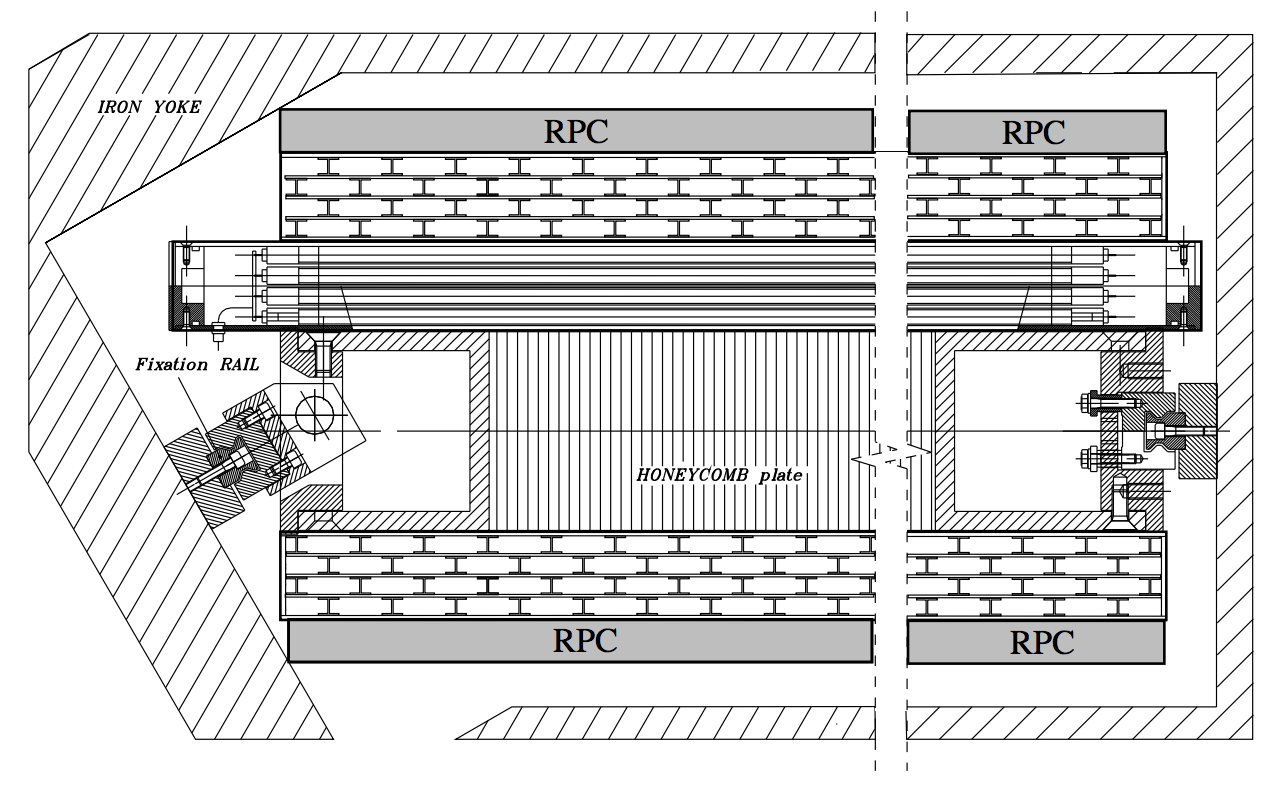
\includegraphics[width=0.8\textwidth]{DT_schematic}
\caption[A schematic drawing of a drift tube chamber.]{A schematic of a drift tube chamber, in the $r-\phi$ plane. Visible are
two cells running parallel to the beamline (immediately above and below the
RPCs) and one cell perpendicular to the beam (above the honeycomb plate).}
\label{fig:DT}
\end{figure}

The CSCs are used in the endcap regions, where the higher flux of particles and 
non-uniformity of the magnetic field make the drift tubes suboptimal. They
consist of a weave of copper cathode strips and anode wires placed within a
volume of gas. Each chamber contains 7 of the cathodes, with 6 planes of wires
running perpendicular across them. The chambers cover 10 or $20^\circ$ of $\phi$
and are staggered in placement to provide full coverage.  Similar to the DTs,
particles moving through the gas result in ionization. The positive ions
produced are pulled toward the negatively charged copper cathodes while the
negatively charged ions are attracted to the positively-charged wires.  As a
result of the fine perpendicular `grid' spacing between the strips and the
wires, the CSCs have a quicker response time than the DTs (CSC pulses last
$\sim 150~ns$, compared to the $\sim 380~ns$ drift time), while maintaining
similar levels of spatial resolution. The overall timing resolution of the CSC
is 7~ns (when utilizing the entire chamber), and its position measurements are
accurate to the 100~$\mu m$ level.

The RPCs are the quickest technology of the muon systems, but provide the
poorest spatial measurements. The chambers consist of two highly resistant
plates separated by a gap filled with gas. An electric field is set up in such a
way that the chambers work in a so-called ``avalanche mode''--when the gas is
ionized by a particle passing through, a cascade of further ionizations occur.
Each RPC detecting element consists of two gaps joined with a common readout
strips between them. The total signal is the combined effect of the two gaps,
providing a higher detection efficiency and lower voltage requirements than a
single-gap setup. Though the spatial resolution of the RPCs is poor in
comparison to the DTs and CSCs (at the 1~cm level), the RPCs have a much
faster response time than the other muon systems, with a time resolution down
to the order of 1~ns. As a result, the RPCs are able to precisely tag which
bunch crossing a given muon came from, making it invaluable in the triggering
process.

\subsection{Data Acquisition and Trigger}
\label{sub:trigger}
The 25 ns design bunch separation means that beam collisions occur with at the
rate of 40~MHz. Because the full detector readout produces on the order of 1 MB
of data per bunch crossing, some 40 TB of potential data is produced in each
second of operation. As it is obviously impossible to store (or readout) such an
enormous amount of data, CMS was designed with a two-stage trigger system to
reduce the rate of stored collisions to a more reasonable (sub-kHz) level. The
filtering must be done in such a way that those events which contain physically
interesting processes are kept, while the uninteresting events are removed. The
Level-1 (L1) trigger is a hardware system that is designed to reduce event rate
to the order of 100 kHz. This subset of the events is then sent to the
High-Level Trigger (HLT), which is a software system implemented on a computing
farm of commercial CPUs. The HLT uses a fuller event reconstruction in order to
make much more involved decisions on the event, resulting in the final filtered
event rate of $\sim 1$~kHz. 

\subsection{L1 Trigger System}
The L1 Trigger system is a hardware system utilizing a mix of FPGAs and 
ASICs. The L1 chain begins locally, where muon chamber track segments or
calorimeter deposits are used to produced Trigger Primitives (TPs).
The TPs are then utilized in a regional calculation, which covers a subsection
of the detector. From the regional stage, a sorted list of objects is passed to
the global trigger subsystems (either the Global Muon Trigger or the Global
Calorimeter Trigger), which determine the highest rank objects from the muon
and calorimeter systems. These are then passed to the Global Trigger (GT), where
there final decision (accept/reject) is made. The accepted events are then
passed to the HLT for further processing. A diagram of the flow through the L1
Trigger system is depicted in Figure~\ref{fig:L1architecture}

\begin{figure}[h]
\centering
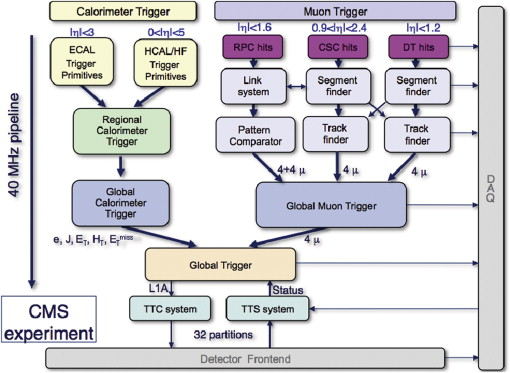
\includegraphics[width=0.7\textwidth]{l1Arch} % source; http://www.sciencedirect.com/science/article/pii/S0168900212009941
\caption[Diagram of the information flow through the CMS trigger system.]{Diagram of the information flow through the CMS trigger system.}
\label{fig:L1architecture}
\end{figure}

\subsubsection{Calorimeter Trigger}
The basic unit in the calorimeter trigger is the trigger tower, corresponding
spatially to a 5$\times$5 grouping of ECAL crystal plus the similarly size HCAL
cell behind it. The energies in each trigger tower are summed by the Trigger
Primitive Generators (TPGs) and passed to the Regional Calorimeter Trigger
(\emph{RCT}) for further processing.  The RCT is made of 18 electronics crates,
each one housing 7 receiver cards and 7 electron identification cards (each of
which provides coverage for two 4$\times$4 regions of trigger towers) and one
jet/summary card. The RCT decompresses the energies reported by the calorimeter
TPGs, and finds the most energetic electron/photon candidates (no distinction
between them is made at this level) within each regions. There are, in addition,
checks to see whether each of these candidates is isolated or not. The RCT
passes the four highest non-isolated candidates, the four highest energy
isolated highest candidates, and the energy sums from each region on to the
Global Calorimeter Trigger (GCT).

As the name suggests, the GCT is the first level at which the calorimeter
information is processed for the entire calorimeter trigger geometry. It uses
this information to compute a number of event-level properties, such as jet
multiplicities, missing transverse energy ($ME_T$), and the scalar jet energy sum
($H_T$). In addition, it finds the highest energy electron/photon candidates
(both isolated and not) and identifies hadronic jets within the calorimeter.
These values are all passed the to GT.

\subsubsection{Muon trigger}
The L1 muon trigger system uses information from all three muon subsystems in
order to maximize the efficiency and background rejection. The CSC and DTs
provide local track segments, which are then combined into regional muon tracks
by their Track Finder systems (CSCTFs and DTTFs). The DT provides coverage in
the barrel region, up to $|\eta| < 1.2$, while the CSCs cover the more forward
regions, $0.9 < |\eta| < 2.4$. The RPC also provide regional
track candidates (with excellent timing resolution) with an $|\eta|$ coverage up
to 1.6. The DT and CSC systems each pass 4 muon candidates to the GMT, while the
RPCs pass a total of 8 (4 from the barrel region and 4 from the endcap region).
Matching between CSC+RPC and DT+RPC candidates ensure that the spatial,
momentum, and timing measurements are optimally efficient for triggering.
This information, consisting primarily of $p_T$, charge, position, and quality
of measurement, is passed to the GT which, in combination with the information
from the GCT, makes a trigger decision based on the event as a whole.

\subsection{HLT System}
After an event is accepted at the L1 level by the GT, it is passed to the
HLT for further processing. Within the HLT, the event goes through 
well-defined reconstruction paths, in order to most quickly comb out those events
which contain potentially interesting physics. Because the event rate coming
through the HLT is still immense (on the order of 100~kHz), the HLT does not
necessarily run a complete event reconstruction--instead it just unpacks and
utilizes the pertinent information, governed by the events' triggers at the L1
level. Because the HLT can utilize more complete snapshots of the event
topology, especially information from the tracker system, it has the ability to
reject a significant subset of events (with fake lepton signals or noisy QCD jet
events), outputting roughly 400~Hz of events for storage.
The triggers utilized in this analysis involve finding two (or more)
isolated leptons above a certain $p_T$ threshold. These are explained in more
detail in Chapter~\ref{chapter:analysis}.
